
\section{Mergeable trees}\noteauthor{Елизаров Никита}
Полное описание всех структур и доказательств можно найти в \cite{georgiadis2011data}.
\subsection{Описание структуры и чего мы хотим от этой структуры}
Будем называть \textbf{упорядоченной кучей} (или просто \textbf{кучей}) дерево, где каждой вершине v сопоставлен \textbf{рациональный} ключ $\mathbf{l(v)},$ со следующим свойством: $l(v)\geqslant l(parent(v)).$

Будем говорить, что $v > w,$ если $l(v) > l(w).$

В данной секции мы будем рассматривать \textbf{лес упорядоченных куч} (то есть не одну такую кучу, а несколько). Мы хотим уметь поддерживать следующие операции:
\begin{itemize}
        \item $parent(v)$~--- узнать, кто является предком $v$;
        \item $root(v)$~--- узнать, кто является корнем дерева, в котором находится $v$;
        \item  $NCA(v, w)$~--- nearest common ancestor: если в одном дереве, то возвращает первого общего предка; если $v$ и $w$~--- не в одном дереве, то возвращает пустое множестве;
        \item $insert(v, x)$~--- создание нового дерева с одной вершиной $v$ и ключом $x;$
        \item $delete(v)$~--- удалить $v,$ если $v$~--- лист;
        \item $link(v, w)$~--- подвесить $v$ к $w,$ причём $v$~--- корень какого-то дерева из леса, а $w$ должна быть в другом дереве. Также $l(v)\geqslant l(w);$
        \item $cut(v)$~--- удалить ребро между $v$ и его родителем; если $v$ является корнем, то ничего не делаем;
       \item $merge(v, w)$~--- если $v$ и $w$ находятся в разных деревьях, то мы сделаем одну операцию $link(root(v), root(w))$ (или $link(root(w), root(v))$, в зависимости от того, какой из корневых ключей больше). Полученное дерево (или изначальное дерево, если $v$ и $w$ были в одном дереве) обозначим за $T$. Тогда нас интересуют два пути:
       \begin{itemize}
           \item $P$~--- путь от $v$ к корню дерева $T$;
           \item $Q$~--- путь от $w$ к корню дерева $T$.
       \end{itemize}
       Мы хотим совместить $P$ и $Q$, чтобы $v$ и $w$ оказались на одном пути от корня $T$ к какому-то листу. При этом, мы хотим, чтобы свойство кучи сохранилось.
       
       Примеры двух \textbf{merge} показаны ниже:
       \begin{figure}[h]
        \center{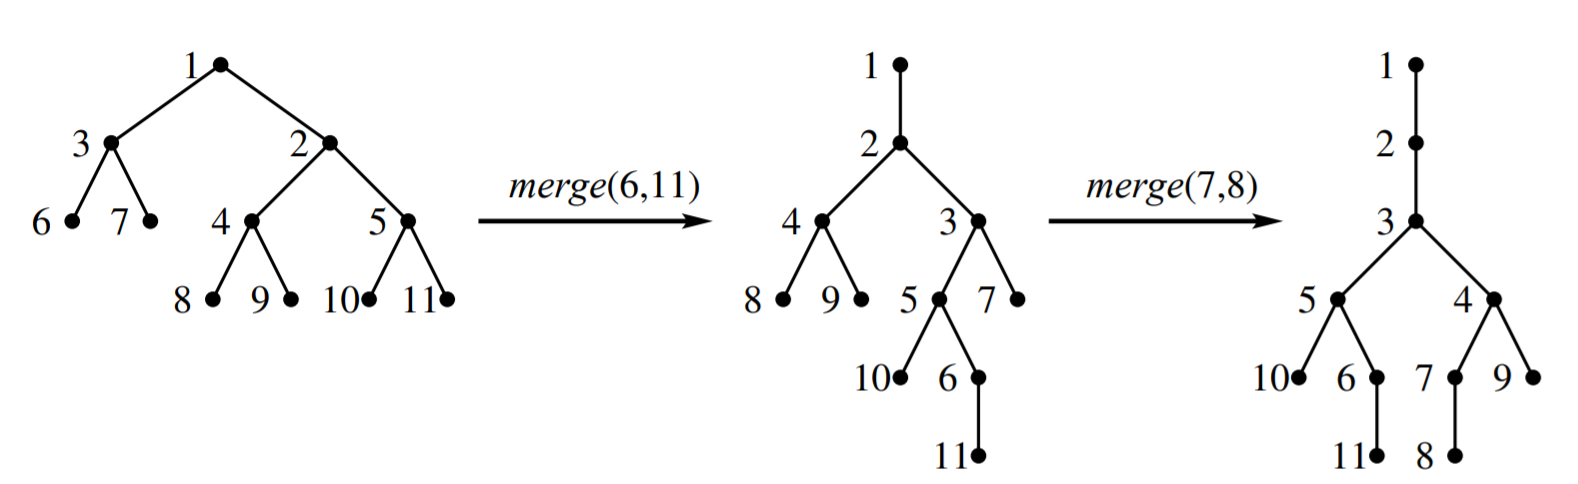
\includegraphics[scale = 0.4]{img/merge.png}}
        \caption{merge}
        \label{fig:image}
        \end{figure}
    \end{itemize}
    
    Теперь поговорим немного про то, как именно мы будем это реализовывать. Мы будем использовать такую же реализацию динамического дерева, как это было в $\mathbf{link-cut\:\:trees}$ (подробнее в предыдущей секции). Тогда все операции, кроме $\mathbf{merge}$ и $\mathbf{NCA}$ мы делать уже умеем. Для реализации $\mathbf{merge}$ нам нужно ввести еще одну операцию~--- $\mathbf{topmost(x, w)}.$
    \begin{itemize}
        \item $topmost(v, w)$~--- возвращает ближайшую к $root(v)$ вершину $t$ на пути $[root(v), v]$, такую, что $l(t) > l(w).$ Предпологается, что $l(v) > l(w).$
    \end{itemize}
    
    Покажем, что мы умеем амортизированно делать $\mathbf{NCA}$ и $\mathbf{topmost}$ за $\mathcal{O}(\log{n}):$
    \begin{algorithmic}[1]
    \Procedure {NCA}{v, u}
        \State{expose(v)}
        \State{expose(w)}
        \State\Return{successor(findTail(v))}
    \EndProcedure
    \end{algorithmic}
    \begin{algorithmic}[1]
    \Procedure {topmost}{v, w}
        \State{expose(v)}
        \State\Return{Binary\_Search(l(w), Splay\_Tree(v))}
    \EndProcedure
    \end{algorithmic}
    
    Здесь $\mathbf{Binary\_Search}(\:\:\cdot\:\:,Splay\_Tree(v))$~--- это бинарный поиск в \textbf{splay-дереве}, которое соответствует сплошному пути, содержащему вершину $\mathbf{v}.$ 
    
    Для полного понимания, нужно вспомнить, что \textbf{splay-дерево} строилось по \guillemotleftнеявным\guillemotright$\:\:$ ключам для пути (а именно: ключом вершины был её порядковый номер в пути). Но, мы будем строить наши \textbf{splay-деревья} по ключам из кучи. В силу того, что на любом пути ключи возрастают, порядок и структура дерева не изменятся.
    
\subsection{Реализация merge}
Для начала заметим, что \textbf{link}~--- это тот же самый \textbf{merge}. Поэтому, будем считать, что все операции \textbf{link} это операции \textbf{merge}.
\begin{algorithmic}[1]
    \Procedure {merge}{v, u}
        \If{root(v)$\ne$ root(w)}
            \If{l(v) $\geqslant$ l(w)}
                \State{link(v, w)}
            \Else
                \State{link(w, v)}
            \EndIf
        \EndIf
        \State {u := NCA(v, w)}\Comment{ищем общего предка v и w}
        \If{u = v or u = w}
            \State \Return{$\varnothing$} \Comment{если общий предок совпадает с v или w, то пути уже совмещены}
        
        \Else 
            \State {x := topmost(v, u)}
            \State {y := topmost(w, u)}
            \If{x < y}\Comment{нужно, потому что будем вставлять на первом шаге}
                \State {swap(x, y)}\Comment{путь от x до v в путь от y до w}
                \State {swap(v, w)}
            \EndIf
            \If {u $\ne$ $\varnothing$}
                \State {cut(x)}
            \EndIf
            \While {x < u} \Comment{начало \textbf{merge step}}
                    \State {t := topmost(w, x)} \Comment{$l(z) \leqslant l(x)$, а l(t) уже нет} 
                    \State{link(x, parent(t))}\Comment{значит x должен быть ребёнком z}
                    \State{cut(t)}
                    \State{y := x} \Comment{теперь мы хотим вставлять путь от t до w}
                    \State{x := t} \Comment{в путь от x до v}
                    \State{swap(v, w)}\Comment{конец \textbf{merge step}}
            \EndWhile
            \State {link(x, w)}
        \EndIf
    \EndProcedure
            
\end{algorithmic}

Операцию, которая находится в теле while назовём \textbf{merge step}. Картинка к ней показана ниже:
\begin{figure}[h]
\center{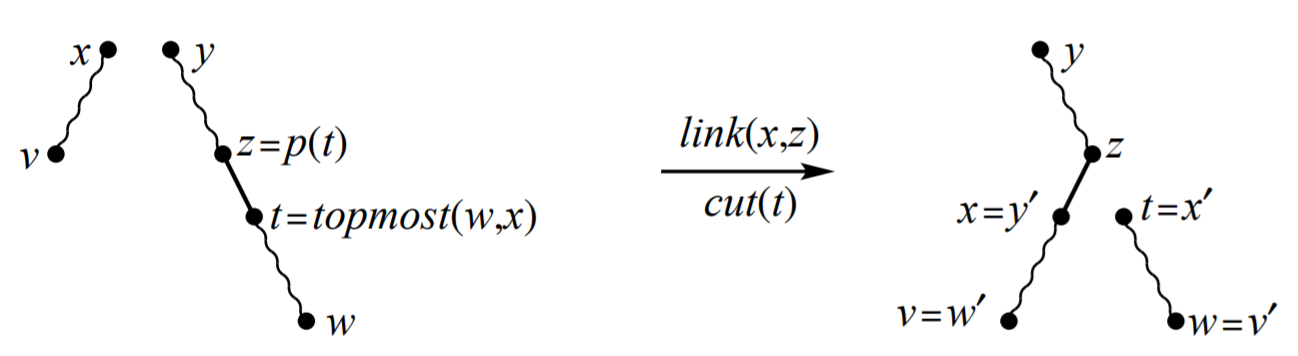
\includegraphics[scale = 0.4]{img/mergestep.png}}
\caption{merge step}
\label{merge step}
\end{figure}


\textbf{Маленький комментарий.} В начале было анонсированно, что куча бинарная. Но в статье я не нашёл этого (плюс, судя по определению $link,$ дерево таки не бинарное). Это вызывает проблему использования $link-cut$ деревьев, так как мы умеем только для бинарных.

Далее, с этого момента, я буду предпологать, что наши деревья небинарные (вроде на небинарные $link-cut$ деревья работают те же оценки). Но, если вдруг, деревья всё-таки бинарные, то мы не всегда можем делать $link,$ особенно для двух корней деревьев. Здесь нам поможет следующий трюк. Давайте не будем искать общего предка. Вместо этого сразу скажем, что один из корней $x,$ а другой $y,$ то есть сразу перейдём к $merge\:\:steps.$\label{trick}

$\quad$

Чтобы оценить количество шагов, достаточно оценить количество изменений родителя какой-либо вершины. Поймём, что количество изменений родителя это количество $\mathbf{merge\:\:steps}$ плюс не более чем 2: в каждом $\mathbf{merge\:\:step}$ ровно одно изменение родителя, еще одно берётся в самом конце~--- в $\mathbf{link(x, w)}$, и еще может быть одно, если они из разных деревьев мы делаем $\mathbf{initial\:\:link}$.

Теперь докажем следующую лемму.
\begin{lemma}\label{first lemm}
Количество изменений родителей за все \textbf{merge}~--- это $\mathcal{O}(m\log{n}).$
\end{lemma}
\begin{proof}
Будем считать, что все наши ключи это не просто рациональные числа, а числа $\{1,\dots n\}.$ Для этого упорядочим все наши ключи в порядке возрастания и заменим каждый ключ на соответствующий номер.

$\quad$

Определим \textbf{cost} операции как количество изменений родителя. 
$$\mathbf{am.\: cost} = cost + \Delta\Phi$$
Потенциал следующий:
\begin{itemize}
    \item каждому ребру $e$ даём 1 потенциала($\Phi_e$);
    \item от каждого ребра $(v, parent(v))$ дадим $\log{(v - parent(v))}$ родителю и $\log{(v - parent(v))}$ ребёнку;
    \item $\Phi_v$ от вершины определяется как сумма потенциалов, которая приходит ей от рёбер (из предыдущего пункта);
    \item $\Phi = \sum\limits_{v\in V}\Phi_v + \sum\limits_{e \in E}\Phi_e.$
    
\end{itemize}
Заметим, что \textbf{cut} и \textbf{delete} уменьшают $\Phi$ хотя бы на 1 и дают не более одного изменения родителя. Значит их $\mathbf{am.\:cost} \leqslant 0.$ Остаётся только \textbf{merge}.

В начале \textbf{merge} возможен \textbf{initial link} (так как вершины могут быть в разных деревьях). Заметим, что он увеличивает потенциал не более, чем на $2\log{n} + 1:$ по $\log{n}$ каждой корневой вершине, которые мы соединяем, и 1 от ребра.

Как влияет \textbf{merge step}:
Посмотрим на родителей $t$ за два \textbf{merge step}: пусть $parent'(t)$ это родитель, который будет у $t$ на следующем \textbf{merge step} после того, который показан на рисунке \ref{merge step}. Тогда:
$$t > parent'(t)\geqslant x > parent(t)$$

Первое неравенство понятно~--- это просто свойство кучи, второе чуть хитрее: новый родитель $t$ будет в ветке $y',$ то есть в ветке $x,$ но вполне может так оказаться, что это будет сам $x,$ поэтому знак нестрогий. Последнее неравенство снова видно из рисунка \ref{merge step}, так как $z = parent(x).$

Математической магией этих трёх неравенств получаем, что:
\begin{enumerate}
    \item либо $t - parent'(t)\leqslant\frac{t - parent(t)}{2};$
    \item либо $x - parent(t)\leqslant \frac{t - parent(t)}{2}.$
\end{enumerate}

Заметим, что гарантированно выполняется одно из этих двух условий. Более того, потенциал меняется только у вершин $t$ и $parent(t).$ Разберём каждое из них:
\begin{enumerate}
    \item Рассмотрим вершину $t.$ Тогда потенциал, приходящий от родителя для неё уменьшается хотя бы на $\log{(t - parent(t))} - \log{(t - parent'(t))} = \log{\frac{t - parent(t)}{t - parent'(t)}}\geqslant 1.$ Потенциал, приходящий от детей для неё не изменился. Где еще произошло изменение потенциала? Мог изменится потенциал, приходиящий от детей для вершины $parent(t):$ он был $\log{(t - parent(t))},$ а стал $\log{(x - parent(t))}.$ Но $t - parent(t) > x - parent(t),$ а значит он снова мог только уменьшиться. Значит одно изменение родителя скомпенсировалось уменьшением потенциала хотя бы на 1.
    
    \item Рассмотрим вершину $parent(t).$ Тогда потенциал, приходящий от детей для неё уменьшается хотя бы на $\log{(t - parent(t))} - \log{(x - parent(t))} = \log{\frac{t - parent(t)}{x - parent(t)}} \geqslant 1.$ Потенциал, приходящий от родителей для неё не меняется. Где еще произошло изменение потенциала? Мог измениться потенциал, приходящий от родителей вершины $t:$ он был $\log{(t - parent(t))},$ а стал $\log{(t - parent'(t))}.$ Но $t - parent(t) > t - parent'(t),$ а значит он снова мог только уменьшиться. Значит одно изменение родителя скомпенсировалось уменьшением потенциала хотя бы на 1.
\end{enumerate}
Таким образом, \textbf{am. cost} за один \textbf{merge} $=\mathcal{O}(\log{n})$. Действительно, \textbf{initial link} даёт нам $2\log{n} + 1$, каждый \textbf{merge step} даёт нам не более 0 и, в конце произолшло одно дополнительное изменение родителя.
\end{proof}

Наконец, итоговое изменение потенциала $\Delta\Phi$ больше нуля, так как в начале был ноль, а в конце что-то положительное. Значит $total\_cost \leqslant total\_am.cost - \Delta\Phi \leqslant total\_am.cost = \mathcal{O}(m\cdot\log{n}).$ Теперь, вспоминая, что все операции в нашем дереве работают за $\mathcal{O}(m\cdot\log(n))$ мы получаем оценку $\mathcal{O}(m\cdot\log^2{n})$ на все операции \textbf{merge}.

\textbf{Маленькое замечание.} Если мы считаем, что все наши деревья бинарные, то нужно заметить, что в трюке, который был упомянут ранее, на первом шаге потенциал также увеличится на $2\log{n} + 1.$ Все остальные \textbf{merge steps} не изменятся.

\subsection{Merge без операций cut}
Теперь мы хотим получить амортизированный $\mathcal{O}(\log{n})$ вместо $\mathcal{O}(\log^2{n}).$ Также как и в прошлой секции, будем представлять дерево в виде объединения непересекающихся по вершинам сплошных путей, соединённых пунктирными рёбрами. 

\newdefn{Определим ранг вершины, как $r(v) := \bigl[\log{size(v)}\bigr],$ где $size(v)$~--- это сумма по ключам в поддереве $v,$ включая саму $v.$}

Ребро $(v, w)$ будет сплошным, если $r(v) = r(w)$. Иначе ребро будет пунктирным. Пример разбиения на пути можно увидеть на рисунке \ref{merge rank}.
\begin{figure}[h]
\center{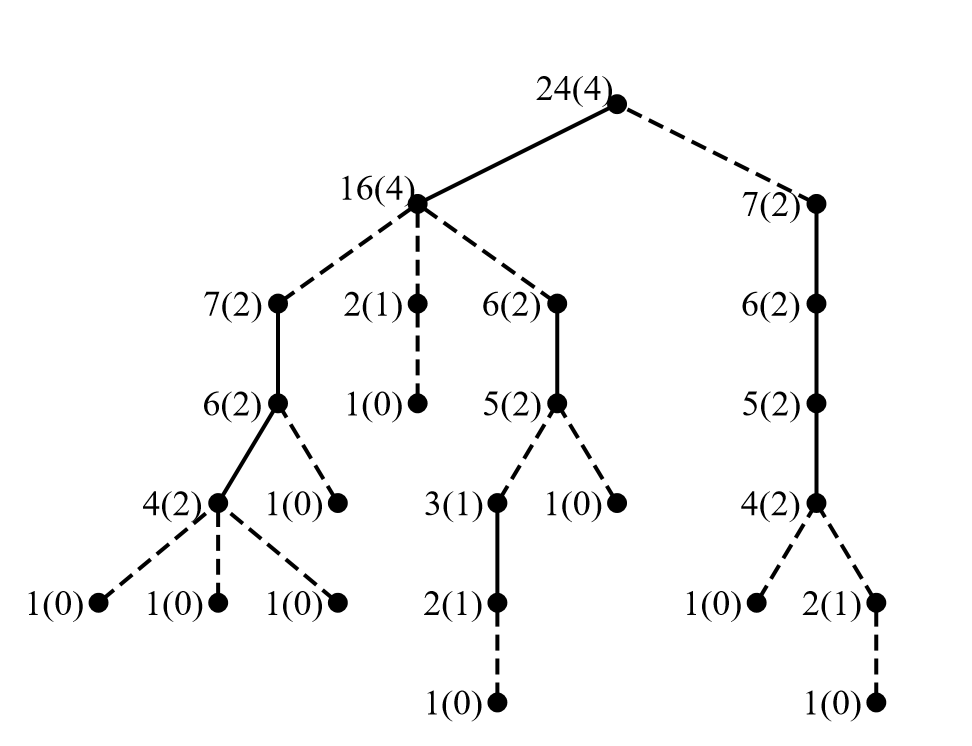
\includegraphics[scale = 0.4]{img/merge_ranks.png}}
\caption{разбиение дерева на пути по рангам}
\label{merge rank}
\end{figure}

Как и в прошлой подсекции, мы считаем, что все ключи это числа $[1,\dots n].$ Из этого следует, что различных рангов не может быть больше, чем $\log{n} + 1.$
\subsubsection{Новая структура дерева}
Для каждого узла будем хранить следующее:
\begin{itemize}
    \item указатель на \textbf{parent(x)};
    \item указатель на \textbf{solid child(x)} (то есть указатель на ребёнка, соединённого сплошным ребром, если такой есть);
    \item указатель на \textbf{head(x)}~--- отдельная вершина, в которой хранится указатель начало сплошного пути (в будущем будем обозначать начало пути как \textbf{top}), в котором вершина находится;
    \item \textbf{dashed size(x)} $:= 1 + \sum\limits_{u \text{~--- пунктирный ребёнок}}size(u)$
\end{itemize}


Также, для каждого сплошного пути мы будем хранить следующее:
\begin{itemize}
    \item \textbf{head(x)}~--- отдельная вершина, в которой хранится указатель на \textbf{top} пути, а также размер \textbf{top} и ранг всего пути (так как в нашем случае ранги у всех вершин из сплошных путей равны~--- это ровно критерий, по которому составлялись сплошные пути);
    \item поисковая структура~--- структура, которая будет уметь выполнять три функции (на ближайшие несколько подподсекций будем считать, что это чёрная коробка, которая просто умеет делать представленные функции):
    \begin{itemize}
        \item удалять узлы в начале пути за $\mathcal{O}(1)$;
        \item добавлять одиночные узлы перед заданным за $\mathcal{O}(1)$;
        \item возвращать \textbf{topnode(x, s)}~--- наименьший узел на сплошном пути, содержащим $s,$ ключ которого больше чем $x.$
    \end{itemize}
    \item более того, каждый \textbf{head} хранит указатель на поисковую структуру соответствующуего сплошного пути.
\end{itemize}

Тот факт, что мы храним только размер \textbf{top} пути, позволяет нам пересчитывать все остальные размеры, пользуясь формулой:
\begin{equation*}
    size(x) = size(parent(x)) - d(parent(x)).
\end{equation*}


На нашем дереве мы хотим поддерживать следующие операции:
\begin{itemize}
    \item $insert(x, w)$~--- просто создаём дерево, состоящее из одной вершины и одного пути. Соответсвенно иницилиазируем поисковую структуру и $head.$ В худшем случае это делается за $\mathcal{O}(1);$
    \item $parent(v)$~--- в нашем случае можно просто перейти по указателю за $\mathcal{O}(1);$
    \item $root(v)$~--- мы немного изменим выход операции $root(v).$ Теперь мы будем возвращать не только сам корень, но стек, состоящий из \textbf{top} всех сплошных путей, которые находятся на $[root(v), v].$ Так как у каждого элемента есть указатель на \textbf{top} своего пути, а также беря в рассмотрение тот факт, что сплошных путей не больше, чем различных рангов (каждому сплошному пути соответсвует ровно один ранг), получаем, что $root(v)$ работает за $\mathcal{O}(\log{n}).$ Будем обозначать выход $root(v)$ за $S_v;$
    \item 
    \begin{algorithmic}[1]
\Procedure{NCA}{v, w}
    \If{$Top(S_w)\ne Top(S_v)$}
        \State\Return {$\varnothing$}
    \Else
        \While{$Top(S_v) = Top(S_w)$}
            \State {$pop(S_v$)}
            \State {$pop(S_w)$}
        \EndWhile
        \If{$S_v = S_w = \varnothing$}
            \State\Return{min\{$v, w$\}}
        \EndIf
        \If {$S_v = \varnothing$ and $S_w\ne\varnothing$}
            \State\Return {min\{$v, parent(Top(S_w))$\}}
        \EndIf
        \If {$S_v \ne \varnothing$ and $S_w = \varnothing$}
            \State\Return {min\{$w, parent(Top(S_v))$\}}
        \EndIf
        \If {$S_v \ne \varnothing$ and $S_w\ne\varnothing$}
            \State\Return {min\{$parent(Top(S_v)), parent(Top(S_w))$\}}
        \EndIf
    \EndIf
\EndProcedure
\end{algorithmic}
Заметим, что размер каждого стека $S_v$ и $S_w$ не превосходит $\log{n} + 1.$ Во время работы \textbf{NCA} мы проходим по стекам $S_v$ и $S_w$ не более раза. Значит \textbf{NCA} работает за  $\mathcal{O}(\log{n}).$
    \item $link(v, w)$~--- рассмотрим отдельно;
    \item $merge(v, w)$~--- рассмотрим отдельно.
\end{itemize}

\subsubsection{Link}
Для начала заметим, что при операции \textbf{link(v,w)}, у каждого предка $w$ увеличивается $size$ на \textbf{size(v)}. Это значит, что у всех сплошных путей выше $w$ $size$ увеличивается одинаково, что облегчает пересчёт их рангов.

Сам \textbf{link} состоит из 4х частей:
\begin{itemize}
    \item сначала добавляем ребро $(v, w)$ как пунктирное ребро;
    \item находим множество $Q$~--- вершины, ранг которых увеличился;
    \item делаем все сплошные рёбра, выходящие из детей вершин из $Q$, пунктирными;
    \item делаем рёбра вершин из $Q\cup \{v\}$ в их родителя сплошными, если у них совпадают ранги.
\end{itemize}
Теперь я постараюсь описать процесс чуть более детально:
\begin{itemize}
    \item находим $S_w,$ делаем $parent(v) = w$ и добавляем $size(v)$ к $d(w)$ и к каждому $size(x),$ где $x\in S_w;$
    \item повторяем следующее, до тех пор, пока $S_w$ не станет пустым: вытаскиваем вернхий элелемент $f\in S_w,$ вычисляем его новый ранг, если ранг увеличился, то добавляем его в конец $Q.$ Если у $f$ есть сплошной ребёнок, то вычисляем его новый $size$ как $size(f) - d(f)$ и пушим $g$ в $S_w.$ Так как ранг вершины не может увеличиться, без увелечения ранга её сплошного родителя, то эта операция корректна;
    \item идём по $Q$ из начала в конец: смотрим на $f\in Q,$ если у $f$ есть сплошной ребёнок $g$, то делаем $solid(f) = null,$ добавляем $size(g)$ к $d(f),$ удаляем $f$ из поисковой структуры $head(g),$ делаем $top(head(g)) = g,$ а $f$ делаем единичным сплошным путём. Мы корректно удаляем всё ненужное из поисковых структур, потому что идём по сплошным путям сверху вниз;
    \item идём по $Q$ из начала в конец: смотрим на $f\in Q,$ если у предка такой же ранг, как и у $f,$ то делаем $solid(parent(f)) = f,$ изменяя при этом $d(parent(f)).$ Далее, удаляем все $head$ и поисковые структуры для $f$ (напомню, $f$~--- одноэлементный сплошной путь), делаем $head(f) = head(parent(f))$ и добавляем $f$ $\guillemotleft$ прямо под $\guillemotright$ $parent(f).$ Если $rank(f) = rank(v),$ то делаем  $head(f) = head(v),$ $top(head(v)) = f$ и добавляем $f$ $\guillemotleft$ прямо над $\guillemotright$ $v.$ Завершающий шаг такой: если $v$ и $w$ имеют одинаковый ранг, то мы делаем ребро между ними сплошным и пересчитываем $d(w).$
\end{itemize}
\begin{lemma}
Суммарное время на все операции \textbf{link} это $\mathcal{O}(m\log{n}).$
\end{lemma}
\begin{proof}
Можем оценить время работы как константа умножить на количество вставок в $Q$ или в $S_w.$ Заметим, что если мы вставляем вершину в $Q,$ то в итоге вставляем и в $S_w$ (когда мы меняем сплошные рёбра на пунктирные; здесь мы можем считать, что мы просто добавляем их в $S_w$). 

Также в самом начале мы вызывали \textbf{root(w)} и поэтому мы добыли $S_w$ размера $\mathcal{O}(\log{n}).$ Заметим, что при добавлении вершины в $S_w$ её ранг увелиличился. Так как ранг для каждой вершины увеличился не более чем на $\mathcal{O}(\log{n})$ раз и $m > n,$ то общее время работы не более $\mathcal{O}(m\cdot\log{n}).$ \textbf{Важно!} Так как у нас нет cut, то ранги только растут.
\end{proof}

\subsubsection{Merge}
Я напишу основную часть алгоритма, но часть про пересчёт структуры я предлагаю прочитать в оригинальной статье (на страницах 12-13 статьи \cite{georgiadis2011data}).

\begin{algorithmic}[1]
    \Procedure {merge}{v, u}
        \If{root(v)$\ne$ root(w)}
            \If{l(v) $\geqslant$ l(w)}
                \State{link(v, w)}
            \Else
                \State{link(w, v)}
            \EndIf
        \EndIf
        \State {u := NCA(v, w)}\Comment{ищем общего предка v и w}
        \If{u = v or u = w}
            \State \Return{$\varnothing$} \Comment{если общий предок совпадает с v или w, то пути уже совмещены}
        
        \Else 
            \State {$S_v$ = root(v)}
            \State {$S_w$ = root(w)}
            \While {$Top(S_v) = Top(S_w)$}
                \State{$pop(S_v)$}
                \State{$pop(S_w)$}
            \EndWhile
            \If {$S_v \ne \varnothing$ and $parent(Top(S_v)) = u$}
                \State{x := $Top(S_v)$}
            \Else
                \State{x := solid(u)}
            \EndIf
            
            \If {$S_w \ne \varnothing$ and $parent(Top(S_w)) = u$}
                \State{y := $Top(S_w)$}
            \Else
                \State{y := solid(u)}
            \EndIf
            
            \If{x < y}
                \State{x := y}
                \State{swap(v, w)}
                \State{$swap(S_v, S_w)$}
            \EndIf
            
            \While {x < w}\Comment{начало \textbf{merge step}}
                z := $Top(S_w)$
                \While {$z\ne null$ and $x > parent(z)$}
                    \State{replace z by the node below it on $S_w$}
                    \State{Make it null if we reached bottom of $S_w$}
                \EndWhile
                \If {z = null}
                    \State{t := topnode(x, w)}
                \Else
                    \State{t := topnode(x, parent(z))}
                \EndIf
                \State{parent(x):=parent(t)}
                \State{\textbf{Update data structure}}
		\State{x := t}
                \State{swap(v, w)}
                \State{swap($S_v, S_w$)}\Comment{конец \textbf{merge step}}
            \EndWhile
        \EndIf
    \EndProcedure
    
\end{algorithmic}
Новый \textbf{merge step} показан на рисунке \ref{new merge}:
\begin{figure}[h]
\center{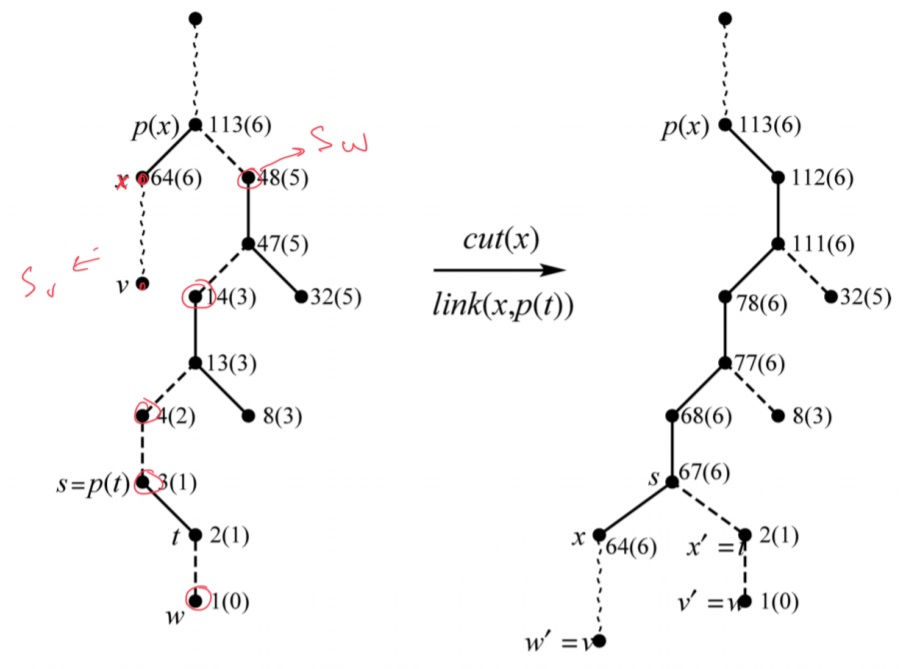
\includegraphics[scale = 0.4]{img/new_merge.png}}
\caption{new merge step}
\label{new merge}
\end{figure}

\textbf{Небольшое замечание.} Для того, чтобы понять следующую лемму, по-хорошему, надо понимать ту самую часть про \textbf{Update data structure}, которую я опустил. Но для леммы достаточно понимать, что мы обновляем снова используя очередь $Q,$ в которую мы добавляем вершины только после того, как достаём их из одного из стеков $S_w$ и $S_v.$

\begin{lemma}
Не считая вызовов \textbf{topnode}, затраченное время на все \textbf{merge} не превосходит $\mathcal{O}(m\cdot\log{n}).$
\end{lemma}
\begin{proof}
Во время одного merge мы возможно соединяем два дерева с помощью \textbf{link}. Это мы делаем за амортизированный $\mathcal{O}(\log{n}).$ 

Если не учитывать \textbf{topnode}, то время, затраченное на $merge$ это $\mathcal{O}(1)$ за каждый \textbf{merge step} плюс $\mathcal{O}(1)$ за каждую вершину, которую мы добавляем в $Q.$

Из первой подсекции (лемма \ref{first lemm}) мы знаем, что количество \textbf{merge steps} это $\mathcal{O}(m\cdot\log{n}.)$ Во время \textbf{merge step} мы достаем из $S_v$ и $S_w$ и добавляем в $Q.$ Как и в прошлой лемме, в начале мы добавили в $S_v$ и $S_w$ по $\mathcal{O}(\log{n})$ вершин, а последующие добавления снова лишь увеличивают ранг, а так как у каждой вершины не более $\mathcal{O}(\log{n})$ увелечений ранга, то мы снова получаем $\mathcal{O}(m\cdot\log{n}).$ \textbf{Важно!} Так как у нас нет \textbf{cut}, то ранги только растут.

\end{proof}

\subsubsection{Поисковая структура на путях}
Мы будем использовать немного прокаченное \textbf{splay tree}. 

\newdefn{Finger~--- узел, посещённый в splay-дереве последний раз.}
Мы доказывали в третей секции (теорема \ref{DynamicFingerTheorem}), что аморитизированная стоимость операций в \textbf{splay}-дереве равна $\mathcal{O}(\log{(d + 1)}),$ где $d = |f' - f|,$ а $f'$ и $f$~--- новый и старый \textbf{fingers}.
\newdefn{$\log{(d + 1)}$~--- время Коула для данной операции.}
У времени Коула есть одно полезное свойство:
\begin{lemma}
Добавление посещения узла между операциями не уменьшает время Коула.
\end{lemma}
\begin{proof}
Лемма 3.4 на странице 16 в статье \cite{georgiadis2011data}.
\end{proof}
Наша цель его амортизировать в нашей структуре. Но возникает одна проблема: в процессе \textbf{link} и \textbf{merge} мы можем несколько раз добавлять вершину вниз нашего дерева и удалять из корня поочередно, что даст нам логарифм высоты дерева (так как расстояние между \textbf{fingers} будет как раз вся высота). А мы хотим получить амортизированно получить $\mathcal{O}(1).$ Поэтому мы будем добавлять все вершины с задержкой. Тогда все \textbf{fingers} будут рядом при добавлениях и удалениях в структуру. Но, тогда \textbf{topnode} будет не просто бинарным поиском, а чуть сложнее.

Хранить эти дополнительные вершины будем следующим образом: на первую вершину сделаем указатель из самой правой вершины \textbf{splay-дерева}. А новые просто будем последовательно добавлять друг за другом.

Реализация \textbf{topnode(x,e)} выглядит следующим образом: мы делаем бинарный поиск $x$ в \textbf{splay-дереве}, для пути для вершины $e$. Тогда ответом будет являться:
\begin{itemize}
    \item либо последний посещённый узел в бинарном поиске;
    \item либо сплошной ребёнок последнего посещённого узла;
    \item либо вершина, которая находится не в дереве.
\end{itemize}
Если это либо первая, либо вторая ситуация, то, мы нашли и делаем \textbf{splay}. Если же это третья ситуация, то мы остановились в самой правой нижней вершине, обозначим её за $y$, делаем \textbf{splay(y)}, а далее просто идём по указателям по вершинам и последовательно находим \textbf{topnode}. Пока мы идём до нашего результата и находим что-то новое~---добавляем это в \textbf{splay-дерево}.

\begin{lemma}
Если поисковая структура это \textbf{splay-дерево} с задержками, как описано выше, то суммарное время на все операции с обновлениемя поисковых структур и на все \textbf{topnode}~--- это $\mathcal{O}(m\cdot\log{n}).$
\end{lemma}
\begin{proof}
Лемма 3.5 на странице 16 в статье \cite{georgiadis2011data}. 
\end{proof}

